
%%%%%%%%%%%%%%%%%%%%%%% file typeinst.tex %%%%%%%%%%%%%%%%%%%%%%%%%
%
% This is the LaTeX source for the instructions to authors using
% the LaTeX document class 'llncs.cls' for contributions to
% the Lecture Notes in Computer Sciences series.
% http://www.springer.com/lncs       Springer Heidelberg 2006/05/04
%
% It may be used as a template for your own input - copy it
% to a new file with a new name and use it as the basis
% for your article.
%
% NB: the document class 'llncs' has its own and detailed documentation, see
% ftp://ftp.springer.de/data/pubftp/pub/tex/latex/llncs/latex2e/llncsdoc.pdf
%
%%%%%%%%%%%%%%%%%%%%%%%%%%%%%%%%%%%%%%%%%%%%%%%%%%%%%%%%%%%%%%%%%%%


\documentclass[runningheads,a4paper]{llncs}

\usepackage{amssymb}
\setcounter{tocdepth}{3}
\usepackage{graphicx}
\usepackage{xcolor}
\usepackage{hyperref}

\newcommand{\keywords}[1]{\par\addvspace\baselineskip
\noindent\keywordname\enspace\ignorespaces#1}

\pagestyle{headings}

\begin{document}

\mainmatter  % start of an individual contribution

% first the title is needed
\title{TELEMETA, Audio web CMS for Ethnomusicological sound archives}

% a short form should be given in case it is too long for the running head
\titlerunning{TELEMETA, Audio web CMS for Ethnomusicological sound archives}

% the name(s) of the author(s) follow(s) next
%
% NB: Chinese authors should write their first names(s) in front of
% their surnames. This ensures that the names appear correctly in
% the running heads and the author index.
%
\author{Thomas Fillon\inst{1} \and Guillaume Pelerin\inst{1}
 \and Jos{\'e}phine Simonnot\inst{2} 
\thanks{This work was partially done inside the DIADEMS project funded by the national french agency ANR }
}
%
\authorrunning{Thomas Fillon \and Guilaume Pellerin \and Jos{\'e}phine Simonnot}
% (feature abused for this document to repeat the title also on left hand pages)

% the affiliations are given next; don't give your e-mail address
% unless you accept that it will be published
\institute{PARISSON, \url{http://www.parisson.com}\\
\url{{thomas.fillon,guillaume.pellerin}@parisson.com}
\and 
CREM, LESC, CNRS UMR 7186, M.A.E. - Universit{\'e} Paris Ouest\\
\url{josephine.simonnot@mae.u-paris10.fr}}

%\toctitle{Lecture Notes in Computer Science}
%\tocauthor{Authors' Instructions}
\maketitle

% Reset Footnote counter after author definition
\setcounter{footnote}{0}


\begin{abstract}
The abstract should summarize the contents of the paper and should
contain at least 70 and at most 150 words. It should be written using the
\emph{abstract} environment.
\keywords{Sound archives, Ethnomusicology, Database, web platform, Metadata}
\end{abstract}


\section{Introduction}

In social sciences like anthropology or linguistic, researchers have to work on multiple type of multimedia documents like photos, videos, sound recordings or databases. The need to easily access, visualize and annotate such materials can be problematic given their diverse formats, sources and given their chronological nature.
This particular concern gets together some laboratories\footnote{the Research Center on Ethnomusicology (CREM), the Musical Acoustics Laboratory (LAM, UMR 7190) and the sound archives of the Mediterranean House of Human Sciences (MMHS)} involved in research on Ethnomusicoly from  the french National Center on Scientific Research (CNRS).

Given those considerations, since 2007, the CREM laboratory and Parisson, a company specialized in the management of audio databases, have been developing \emph{Telemeta}, an innovative, collaborative and interdisciplinary open web-based multimedia platform that fits the professional requirements from both sound archivists and researchers in ethnomusicology. Since 2008, a first prototype of this platform has been online\footnote{Archives sonores du CNRS, Musée de l'Homme, \url{http://archives.crem-cnrs.fr}}.

%With the help and expertise of Parisson, a company specialized in the management of audio database, a first prototype of this web-based multimedia platform, named \emph{Telemeta} has been online since 2008 and enable to access sound archives of the CREM laboratory and their associated documentations \cite{telemetaCREM}.%\footnote{Archives sonores du CNRS, Musée de l'Homme, \url{http://archives.crem-cnrs.fr}}


%Accessing audio archives materials with numerous collection of items of arbitrary duration ranging from a minute to several hours was a common issue shared by some laboratories from the french National Center on Scientific Research (CNRS) and involved in research on Ethnomusicoly. Those laboratories, the Research Center on Ethnomusicology (CREM),the Musical Acoustics Laboratory (LAM, UMR 7190) and the sound archives of the Mediterranean House of Human Sciences (MMHS) have decided to join together to develop a solution for managing, preserving, accessing and broadcasting their sound archives.



\section{Telemeta}\label{sec:Telemeta}
\subsection{Web audio content management features and architecture}
Telemeta\footnote{\url{http://telemeta.org}} is a free and open source\footnote{Telemeta code is available under the \href{http://cecill.info/licences/Licence_CeCILL_V2-en.html}{CeCILL Free Software License Agreement}} web audio content management system which introduces useful and secure methods to backup, index, transcode, analyse and publish any digitalized audio file with its metadata. 

An overview of the Telemeta's web interface is illustrated in Figure~\ref{fig:Telemeta}

\begin{figure}[htbp]
  \centering
  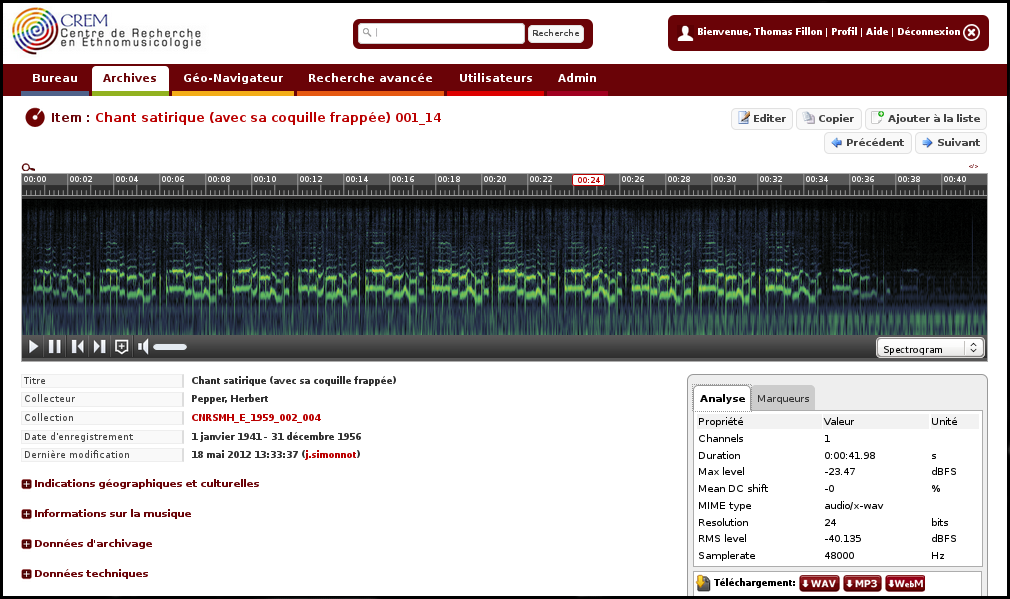
\includegraphics[width=10cm]{img/telemeta.png}
  \caption{Screenshot excerpt of the \emph{Telemeta} web interface}\label{fig:Telemeta}
\end{figure}

Telemeta is dedicated to professionals who wants to easily organize, backup, archive and publish documented sound collections of audio files, CDs, digitalized vinyls and magnetic tapes over a strong database, in accordance with open web standards. 


\emph{Telemeta} architecture is flexible and can easily be adapted to particular database organization of a given sound archives. 
%\emph{Telemeta} features multi-criteria text-based search engine and functions to easily navigate inside an audio item.
%+ audio analysis (via TimeSide)
%+ time markers for annotation and segmentation of instant or temporal region of the audio data.

Regarding web aspects, the main features of \emph{Telemeta} are :
\begin{itemize}
\item \emph{Pure HTML} web user interface including high level \emph{search engine}
\item Smart \emph{workflow management} with contextual user lists, profiles and rights
  % \item RSS and JSON feed generators
  % \item XML serialized backup
\item Strong SQL or Oracle backend
\item MVC architecture 
\end{itemize}

  

Beside database management, the audio support is mainly provided through an external component : TimeSide which is described in Section~\ref{sec:Timeside}

\subsection{Metadata}\label{sec:metadata}
In addition to the audio data, an efficient and dynamic management of the associated metadata is also required. %Consulting metadata provide both an exhaustive access to valuable information about the source of the data and to the related work of peer researchers. 
Dynamically handling metadata in a collaborative manner enable to optimize the continuous process of knowledge gathering and enrichment of the materials in the database.  
%One of the major challenge is thus the standardization of audio and metadata formats with the aim of long-term preservation and usage of the different materials.
The compatibility with other systems is facilitated by the integration of the metadata standards protocols \emph{Dublin Core} and \emph{OAI-PMH} \cite{DublinCore,OAI-PMH}.

Metadata provide two different kinds of information about the audio item : contextual information and annotations.

\paragraph{Contextual Information}
Regarding ethnomusicology, contextual information could be geographic, cultural and musical. It could also store archives related information and include related materials in any multimedia format.  
\paragraph{Annotation and segmentation}
Metadata also consist in temporal information such as \emph{time-coded makers} with comments and \emph{segmentation} according to ontology relevant for ethnomusicology (e.g. speech versus singing voice segment, chorus, ...)
It should be notice that those annotations and segmentation can be done either by an human expert or by some audio processing automatic analysis (see Section~\ref{sec:Timeside}).


\section{TimeSide}\label{sec:Timeside}
One specificity of the Telemeta architecture is to rely on an external component, \emph{TimeSide}, that offers audio player integration together with audio signal processing analysis capabilities.
 
Figure~\ref{fig:TimeSide_Archi} illustrates the overall architecture of \emph{TimeSide}.

\begin{figure}[htbp]
  \centering
  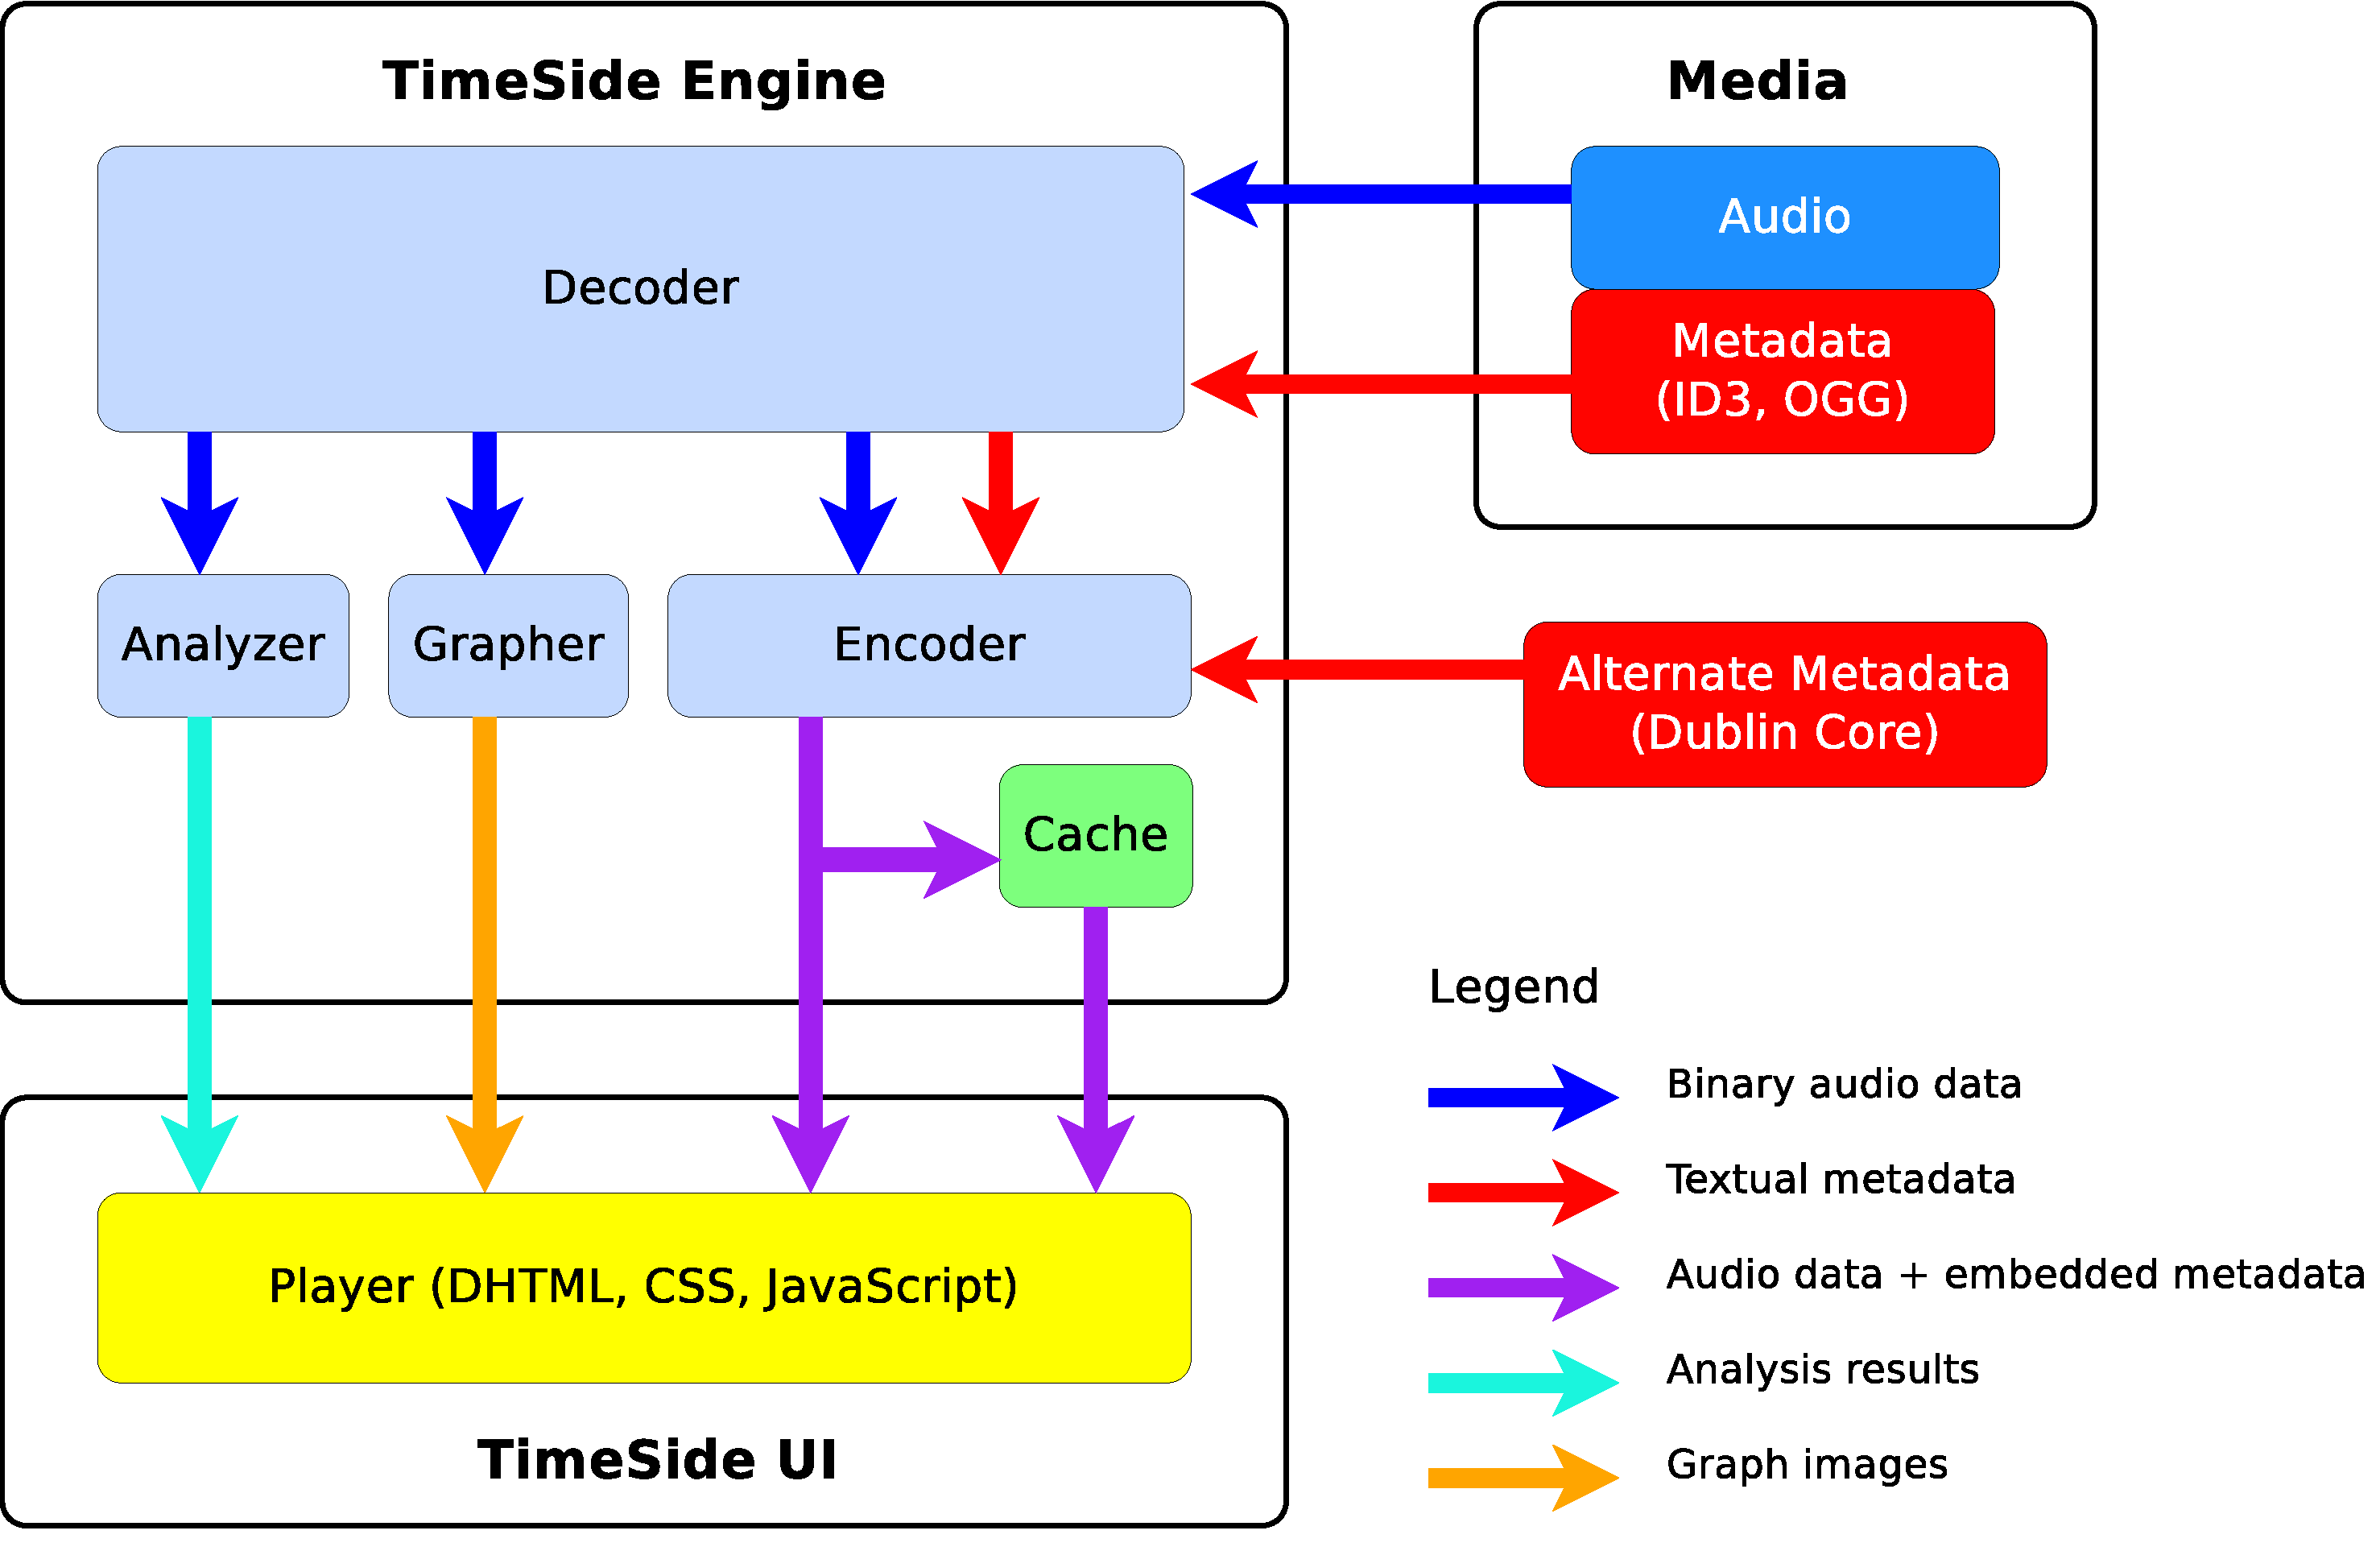
\includegraphics[width=10cm]{img/timeside_schema.pdf}
  \caption{TimeSide architecture}\label{fig:TimeSide_Archi}
\end{figure}


\subsection{Audio management}
TimeSide provides the following main features :
\begin{itemize}
\item \emph{Secure archiving, editing and publishing of audio files} over
  internet.
\item Smart \emph{audio player} with enhance visualization (waveform, spectrogram)
\item \emph{Multi-format support} : read all available audio and video formats  through Gstreamer, transcoding with smart streaming and caching methods% (FLAC, OGG, MP3, WAV and WebM)
  % \item \emph{Playlist management} for all users with CSV data export
\item "On the fly" \emph{audio analyzing, transcoding and metadata
    embedding} based on an easy plugin architecture
\end{itemize}

\subsection{Audio features extraction}
TimeSide incorporates some state-of-the-art audio feature extraction libraries such as Aubio, Yaafe and Vamp plugins \cite{brossierPhD,yaafe_ISMIR2010,vamp-plugins}.
This feature extraction capability enable to automatically analyzes every sound items in a given collection and display the results as a support to ethnomusicological studies.
Further works on that subject will incorporate advance Music Information Retrieval methods to provide automatic annotation and segmentation together with similarity analysis.

\section{Conclusion - Purpose of the demonstration}
The demonstration aims at presenting the features offered by \emph{Telemeta} as detailed in Section~\ref{sec:Telemeta} in the context of ethnomusicological sound archives \cite{telemetaCREM}. It focuses on the enhance and collaborative user-experience for accessing the audio items and associated metadata and on the possibility for the expert user to further enrich those metadata.
Another goal of this demonstration is to present the integrated audio analysis tools described in Section~\ref{sec:Timeside}


\subsubsection*{Acknowledgments.} 
The authors would like to thanks all the people that have been involved in \emph{Telemeta} specification and development or have provide appreciated thoughts during discussions.



\bibliographystyle{splncs03}
\bibliography{cmmr_2013}


\end{document}
